\section{Точечная примесь}
\subsection{Энергия связанных состояний}
Гамильтониан примеси в модели сильной связи, описанной выше, можно записать в виде
\begin{equation}
    V = \Delta E (a_{00}^\dagger a_{00} + b_{00}^\dagger b_{00})
\end{equation}
Связанные состояния даются уравнением
\begin{equation}    
    \det{\left[\mathbbm{1} - \Delta E \int \frac{d^2 p}{(2\pi)^2} 
            \frac{\omega + \hat{H}}{\omega^2 - E_p^2}\right]} = 1
\end{equation}
В последнем интеграле (от матрицы) недиагональные члены из--за симметрии обращаются в ноль.
Таким образом, связанные состояния сводятся к уравнениям
\begin{align}
        &G(\omega,0,0)_{11} = \int \frac{d^2 p}{(2\pi)^2} 
            \frac{\omega + \xi + \frac{1}{m}(2 - \cos{p_x} - \cos{p_y})}
                 {\omega^2 - E_p^2} =\frac{1}{\Delta E}, \label{local_state_eq:1}\\
        &G(\omega,0,0)_{22} = \int \frac{d^2 p}{(2\pi)^2} 
            \frac{-\omega + \xi + \frac{1}{m}(2 - \cos{p_x} - \cos{p_y})}
                 {\omega^2 - E_p^2} =-\frac{1}{\Delta E}, \label{local_state_eq:2}
\end{align}
Эти интегралы можно взять приближённо в круге радиуса $p_{\mathrm{max}}$,
если учесть, что при малых $p$ спектр близок к 
коническому. Можно считать, что $p_{\mathrm{max}} \sim 1$. После интегрирования получается
\begin{equation}
    \label{approx_green_func}
    G(\omega,0,0)_{11} = -\frac{1}{8\pi}\frac{1}{m(4t^2 + \frac{\xi}{m})}
        \left[ p_{\mathrm{max}}^2 + 
            \left(2m(\omega+\xi) - \frac{\xi^2 - \omega^2}{4t^2 + \frac{\xi}{m}}\right) 
                \log{\left(1 + \frac{\left(4t^2 + \frac{\xi}{m}\right)p_{\mathrm{max}}^2}
                                    {\xi^2 - \omega^2}\right)}\right]
\end{equation}
Используя это выражение, можно решить уравнения \eqref{local_state_eq:1} 
на связанные состояния. Оказывается, 
что для $\xi < 0$ связанные состояния в запрещённой зоне существуют для сколь угодно 
глубокой ямы. Для $\xi > 0$ это не так.

Будем решать уравнение \eqref{local_state_eq:1}, 
используя приближение \eqref{approx_green_func}. 
Сделаем предположение, что $\omega = \xi + \delta \omega$, где $|\delta \omega| \ll |\xi|$
(ответ покажет, что это предположение почти всегда выполняется). Тогда можно выкинуть малые 
поправки из приближённого выражения для функции Грина \eqref{approx_green_func}. Получается
уравнение
\begin{equation}
    \label{approx_green_func_1}
    G(\omega,0,0)_{11} = -\frac{1}{8\pi}\frac{1}{m(4t^2 + \frac{\xi}{m})}
        \left[ p_{\mathrm{max}}^2 + 
             4m\xi\log{\left(1 + \frac{\left(4t^2 + \frac{\xi}{m}\right)p_{\mathrm{max}}^2}
                                    {-\xi\,\delta \omega}\right)}\right] = \frac{1}{\Delta E}
\end{equation}
Рассмотрим случай большого $\Delta E$. В этом случае очевидно, что при $\xi > 0$ решений
уравнения \eqref{approx_green_func_1} нет, так как $\delta \omega < 0$ и логарифм в формуле ---
большое положитальное число. Для $\xi < 0$, напротив, логарифм приобретает знак минус, 
и получается решение 
\begin{equation} 
    \delta \omega \approx \frac{\left(4t^2 + \frac{\xi}{m}\right)p_{\mathrm{max}}^2}{|\xi|}
            \exp\left\{ -\frac{p_{\mathrm{max}}^2}{4m|\xi|} - 
                        \frac{8\pi}{4m^2|\xi|\Delta E\left(4t^2 + \frac{\xi}{m}\right)}\right\}
\end{equation}
Уравнение \eqref{local_state_eq:2} переходит в \eqref{local_state_eq:1}  при замене 
$\omega \to -\omega$, $\Delta E \to -\Delta E$.

Интегралы из \eqref{local_state_eq:1},\eqref{local_state_eq:2} 
можно взять численно. Для 
$\xi, m, t = -0.03, 0.1, 0.5$ на графике изображены найденные численно уровни энергии.
Экспоненциальные хвосты на этом графике хорошо видны.

\begin{figure}[h]
    \centering
    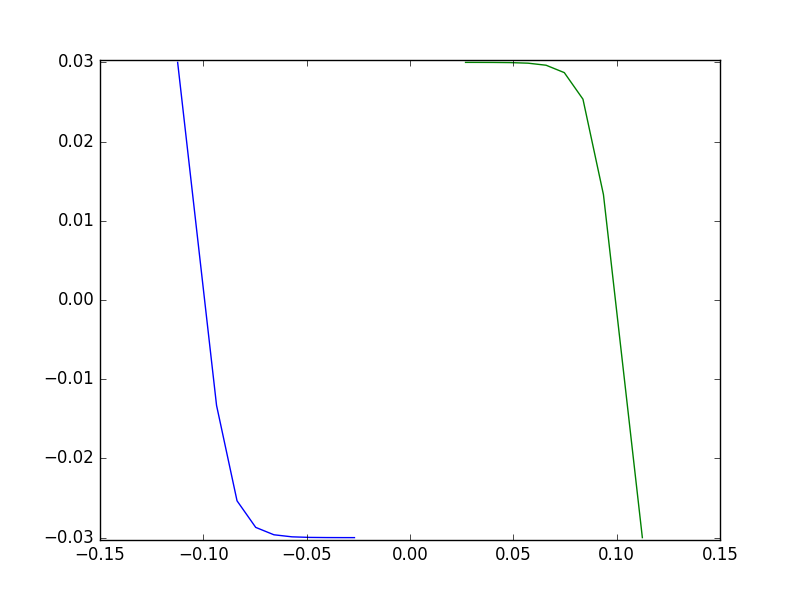
\includegraphics[width=0.8\linewidth]{impurity_levels.png}
    \caption{
            На графике показаны уровни энергии связанных состояний на точечной примеси. 
            По оси абсцисс отложена обратная глубина ямы, $\Delta E^{-1}$. <<Хвосты>>
            обоих графиков должны быть продолжены до бесконечности, у синего графика ---
            вправо снизу, у зелёного --- влево сверху. Видно,
            что при бесконечной глубине ямы имеются два слабо связанных состояния.
            }
\end{figure}

\subsection{Волновые функции}
Волновые функции даются компонентами свободной
функции Грина:
\begin{equation}
    \Psi_{\alpha, i}(x) = G_0(x)_{\alpha i}
\end{equation}
Здесь $\alpha$ --- ``спинорный'' индекс, а $i$ --- индекс, соответствующий номеру волновой 
функции.

Функция Грина --- 
\begin{equation}
    G_0(x) = \int \frac{d^2 p}{(2\pi)^2} 
            \frac{\omega + \hat{H}}{\omega^2 - E_p^2} e^{ipx}
\end{equation}
Их можно вычислить с помощью формального трюка. Определим новую функцию
$F(x,y)$:
\begin{equation}
    F(x,y) = \equiv \int \frac{d^2 p}{(2\pi)^2} 
            \frac{e^{ip_x x + ip_y y}}{\omega^2 - E_p^2} 
\end{equation}
Несложно понять, что компоненты функций Грина выражаются (точными соотношениями)
 через $F(x,y)$. А именно,
\begin{equation}
    \label{differences}
    \begin{split}
        G_{11} & = (\omega + \xi) F(x,y) - 
            \frac{1}{m}(F(x+1,y) + F(x-1,y) + F(x,y+1) + F(x, y-1) - 4F(x,y))\\
        G_{21} & = -it(F(x+1,y) - F(x-1,y)) + t(F(x,y+1) - F(x,y-1))
    \end{split}
\end{equation}
С другой стороны, $F(x,y)$ может быть вычислена приближённо. Если разложить 
выражение в знаменателе около $p = 0$ и распространить интегрирование до $\infty$, то получится
сходящийся и берущийся интеграл.
\begin{equation}
    F(x,y) \approx -\int \frac{p\,dp\,d\cos{\theta}}{(2\pi)^2} 
        \frac{e^{ipr\cos{\theta}}}{\xi^2 - \omega^2 - (4t^2 + \frac{\xi}{m})p^2} = 
        -\frac{1}{2\pi} \frac{1}{4t^2 + \frac{\xi}{m}}
        K_0 \left(\sqrt{\frac{\xi^2 - \omega^2}{4t^2 + \frac{\xi}{m}}}R \right)
\end{equation}
Разности \eqref{differences} можно аппроксимировать производными. Пользуясь тем, что
$K_0(x)$ --- решение модифицированного уравнения Бесселя, получим 
\begin{equation}
    \begin{split}
        G_{11} & = -\frac{1}{2\pi} \frac{1}{4t^2 + \frac{\xi}{m}}
        \left( \omega + \xi - \frac{1}{m} \frac{\xi^2 - \omega^2}{4t^2 + \frac{\xi}{m}} \right)
        K_0 \left(\sqrt{\frac{\xi^2 - \omega^2}{4t^2 + \frac{\xi}{m}}}R \right)\\
        G_{21} & = \frac{it}{\pi} \sqrt{\frac{\xi^2 - \omega^2}
                                     {(4t^2 + \frac{\xi}{m})^{3}}}
        K_0' \left(\sqrt{\frac{\xi^2 - \omega^2}{4t^2 + \frac{\xi}{m}}}R \right)e^{i\theta}
    \end{split}
\end{equation}
%Найдём момент импульса найденных состояний. Оператор полного момента имеет вид
%\begin{equation}
%    J_z = x p_y - y p_x + \frac{1}{2}\sigma_z
%\end{equation}
%Несложно понять, что у двух найденных состояний полный момент равен $\pm \frac{1}{2}$.
%
%Интересно также найти магнитный момент. Оператор магнитного момента ---
%\begin{equation}
%    m_z = \frac{e}{2c}(x v_y - y v_x) + \frac{e}{2m_0c} \sigma_z
%\end{equation}
%Операторы скорости в низшем порядке по импульсам ---
%\begin{equation}
%    \begin{split}
%        v_x & = \begin{pmatrix} 
%                -\frac{i}{m} \partial_ x & 2t \\
%                2t & \frac{i}{m}\partial_x
%              \end{pmatrix} \\
%        v_y & = \begin{pmatrix} 
%                -\frac{i}{m} \partial_y & -2it \\
%                2it & \frac{i}{m}\partial_y
%              \end{pmatrix} \\
%    \end{split}
%\end{equation}
%Таким образом,
%\begin{equation}
%    m_z = \frac{e}{2mc}
%            \begin{pmatrix}
%               l_z & -2imt\cdot re^{-i\theta} \\
%               2imt\cdot r e^{i\theta} & -l_z
%            \end{pmatrix} + 
%          \frac{e}{2m_0c} \sigma_z
%\end{equation}
